\documentclass[a4paper]{report}
% Some basic packages
\usepackage[utf8]{inputenc}
\usepackage[T1]{fontenc}
\usepackage{textcomp}
\usepackage[english]{babel}
\usepackage{url}
\usepackage{graphicx}
\usepackage{float}
\usepackage{booktabs}
\usepackage{enumitem}

\pdfminorversion=7

% Don't indent paragraphs, leave some space between them
\usepackage{parskip}

% Hide page number when page is empty
\usepackage{emptypage}
\usepackage{subcaption}
\usepackage{multicol}
\usepackage{xcolor}

% Other font I sometimes use.
% \usepackage{cmbright}

% Math stuff
\usepackage{amsmath, amsfonts, mathtools, amsthm, amssymb}
% Fancy script capitals
\usepackage{mathrsfs}
\usepackage{cancel}
% Bold math
\usepackage{bm}
% Some shortcuts
\newcommand\N{\ensuremath{\mathbb{N}}}
\newcommand\R{\ensuremath{\mathbb{R}}}
\newcommand\Z{\ensuremath{\mathbb{Z}}}
\renewcommand\O{\ensuremath{\emptyset}}
\newcommand\Q{\ensuremath{\mathbb{Q}}}
\newcommand\C{\ensuremath{\mathbb{C}}}
\renewcommand\L{\ensuremath{\mathcal{L}}}

% Package for Petri Net drawing
\usepackage[version=0.96]{pgf}
\usepackage{tikz}
\usetikzlibrary{arrows,shapes,automata,petri}
\usepackage{tikzit}
\input{petri_nets_style.tikzstyles}

% Easily typeset systems of equations (French package)
\usepackage{systeme}

% Put x \to \infty below \lim
\let\svlim\lim\def\lim{\svlim\limits}

%Make implies and impliedby shorter
\let\implies\Rightarrow
\let\impliedby\Leftarrow
\let\iff\Leftrightarrow
\let\epsilon\varepsilon

% Add \contra symbol to denote contradiction
\usepackage{stmaryrd} % for \lightning
\newcommand\contra{\scalebox{1.5}{$\lightning$}}

% \let\phi\varphi

% Command for short corrections
% Usage: 1+1=\correct{3}{2}

\definecolor{correct}{HTML}{009900}
\newcommand\correct[2]{\ensuremath{\:}{\color{red}{#1}}\ensuremath{\to }{\color{correct}{#2}}\ensuremath{\:}}
\newcommand\green[1]{{\color{correct}{#1}}}

% horizontal rule
\newcommand\hr{
    \noindent\rule[0.5ex]{\linewidth}{0.5pt}
}

% hide parts
\newcommand\hide[1]{}

% si unitx
\usepackage{siunitx}
\sisetup{locale = FR}

% Environments
\makeatother
% For box around Definition, Theorem, \ldots
\usepackage{mdframed}
\mdfsetup{skipabove=1em,skipbelow=0em}
\theoremstyle{definition}
\newmdtheoremenv[nobreak=true]{definitie}{Definitie}
\newmdtheoremenv[nobreak=true]{eigenschap}{Eigenschap}
\newmdtheoremenv[nobreak=true]{gevolg}{Gevolg}
\newmdtheoremenv[nobreak=true]{lemma}{Lemma}
\newmdtheoremenv[nobreak=true]{propositie}{Propositie}
\newmdtheoremenv[nobreak=true]{stelling}{Stelling}
\newmdtheoremenv[nobreak=true]{wet}{Wet}
\newmdtheoremenv[nobreak=true]{postulaat}{Postulaat}
\newmdtheoremenv{conclusie}{Conclusie}
\newmdtheoremenv{toemaatje}{Toemaatje}
\newmdtheoremenv{vermoeden}{Vermoeden}
\newtheorem*{herhaling}{Herhaling}
\newtheorem*{intermezzo}{Intermezzo}
\newtheorem*{notatie}{Notatie}
\newtheorem*{observatie}{Observatie}
\newtheorem*{exe}{Exercise}
\newtheorem*{opmerking}{Opmerking}
\newtheorem*{praktisch}{Praktisch}
\newtheorem*{probleem}{Probleem}
\newtheorem*{terminologie}{Terminologie}
\newtheorem*{toepassing}{Toepassing}
\newtheorem*{uovt}{UOVT}
\newtheorem*{vb}{Voorbeeld}
\newtheorem*{vraag}{Vraag}

\newmdtheoremenv[nobreak=true]{definition}{Definition}
\newtheorem*{eg}{Example}
\newtheorem*{notation}{Notation}
\newtheorem*{previouslyseen}{As previously seen}
\newtheorem*{remark}{Remark}
\newtheorem*{note}{Note}
\newtheorem*{problem}{Problem}
\newtheorem*{observe}{Observe}
\newtheorem*{property}{Property}
\newtheorem*{intuition}{Intuition}
\newmdtheoremenv[nobreak=true]{prop}{Proposition}
\newmdtheoremenv[nobreak=true]{theorem}{Theorem}
\newmdtheoremenv[nobreak=true]{corollary}{Corollary}

% End example and intermezzo environments with a small diamond (just like proof
% environments end with a small square)
\usepackage{etoolbox}
\AtEndEnvironment{vb}{\null\hfill$\diamond$}%
\AtEndEnvironment{intermezzo}{\null\hfill$\diamond$}%
% \AtEndEnvironment{opmerking}{\null\hfill$\diamond$}%

% Fix some spacing
% http://tex.stackexchange.com/questions/22119/how-can-i-change-the-spacing-before-theorems-with-amsthm
\makeatletter
\def\thm@space@setup{%
  \thm@preskip=\parskip \thm@postskip=0pt
}


% Exercise 
% Usage:
% \exercise{5}
% \subexercise{1}
% \subexercise{2}
% \subexercise{3}
% gives
% Exercise 5
%   Exercise 5.1
%   Exercise 5.2
%   Exercise 5.3
\newcommand{\exercise}[1]{%
    \def\@exercise{#1}%
    \subsection*{Exercise #1}
}

\newcommand{\subexercise}[1]{%
    \subsubsection*{Exercise \@exercise.#1}
}


% \lecture starts a new lecture (les in dutch)
%
% Usage:
% \lecture{1}{di 12 feb 2019 16:00}{Inleiding}
%
% This adds a section heading with the number / title of the lecture and a
% margin paragraph with the date.

% I use \dateparts here to hide the year (2019). This way, I can easily parse
% the date of each lecture unambiguously while still having a human-friendly
% short format printed to the pdf.

\usepackage{xifthen}
\def\testdateparts#1{\dateparts#1\relax}
\def\dateparts#1 #2 #3 #4 #5\relax{
    \marginpar{\small\textsf{\mbox{#1 #2 #3 #5}}}
}

\def\@lecture{}%
\newcommand{\lecture}[3]{
    \ifthenelse{\isempty{#3}}{%
        \def\@lecture{Lecture #1}%
    }{%
        \def\@lecture{Lecture #1: #3}%
    }%
    \subsection*{\@lecture}
    \marginpar{\small\textsf{\mbox{#2}}}
}



% These are the fancy headers
\usepackage{fancyhdr}
\pagestyle{fancy}

% LE: left even
% RO: right odd
% CE, CO: center even, center odd
% My name for when I print my lecture notes to use for an open book exam.
% \fancyhead[LE,RO]{Gilles Castel}

\fancyhead[RO,LE]{\@lecture} % Right odd,  Left even
\fancyhead[RE,LO]{}          % Right even, Left odd

\fancyfoot[RO,LE]{\thepage}  % Right odd,  Left even
\fancyfoot[RE,LO]{}          % Right even, Left odd
\fancyfoot[C]{\leftmark}     % Center

\makeatother




% Todonotes and inline notes in fancy boxes
\usepackage{todonotes}
\usepackage{tcolorbox}

% Make boxes breakable
\tcbuselibrary{breakable}

% Verbetering is correction in Dutch
% Usage: 
% \begin{verbetering}
%     Lorem ipsum dolor sit amet, consetetur sadipscing elitr, sed diam nonumy eirmod
%     tempor invidunt ut labore et dolore magna aliquyam erat, sed diam voluptua. At
%     vero eos et accusam et justo duo dolores et ea rebum. Stet clita kasd gubergren,
%     no sea takimata sanctus est Lorem ipsum dolor sit amet.
% \end{verbetering}
\newenvironment{verbetering}{\begin{tcolorbox}[
    arc=0mm,
    colback=white,
    colframe=green!60!black,
    title=Opmerking,
    fonttitle=\sffamily,
    breakable
]}{\end{tcolorbox}}

% Noot is note in Dutch. Same as 'verbetering' but color of box is different
\newenvironment{noot}[1]{\begin{tcolorbox}[
    arc=0mm,
    colback=white,
    colframe=white!60!black,
    title=#1,
    fonttitle=\sffamily,
    breakable
]}{\end{tcolorbox}}




% Figure support as explained in my blog post.
\usepackage{import}
\usepackage{xifthen}
\usepackage{pdfpages}
\usepackage{transparent}
\newcommand{\incfig}[1]{%
    \def\svgwidth{\columnwidth}
    \import{./figures/}{#1.pdf_tex}
}

% Fix some stuff
% %http://tex.stackexchange.com/questions/76273/multiple-pdfs-with-page-group-included-in-a-single-page-warning
\pdfsuppresswarningpagegroup=1


% My name
\author{Bruno M. Pacheco}

 
\begin{document}
 
\title{Laboratório 2}
\author{Bruno M. Pacheco (16100865)\\
Pedro Y. F. Ceripes (18100681) \\
EEL 7550 - Eletrônica Aplicada}
 
\maketitle

\section*{Objetivo}
 
Os experimentos executados visam desenvolver familiaridade e experiência com o uso de amplificadores operacionais em montagem de circuitos comparadores e amplificadores.
 
\section*{Simulações}

\subsection*{Circuito 1}

Conforme requisitado, foi montado o circuito representado pela figura \ref{fig:figures-lab2-1-circuito-png}.

\begin{figure}[H]
    \centering
    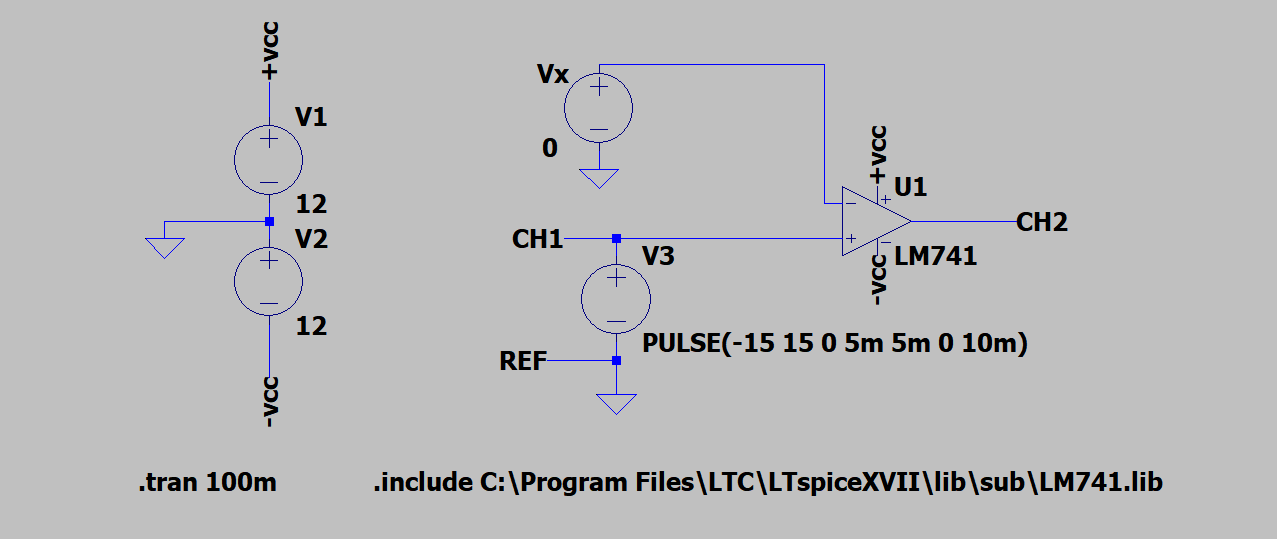
\includegraphics[width=0.9\textwidth]{figures/lab2-1-circuito.png}
    \caption{Primeiro circuito do roteiro.}
    \label{fig:figures-lab2-1-circuito-png}
\end{figure}

\subsubsection*{a)}

O resultado da simulação pode ser visualizado na figura \ref{fig:figures-lab2-1-a-png}.

\begin{figure}[H]
    \centering
    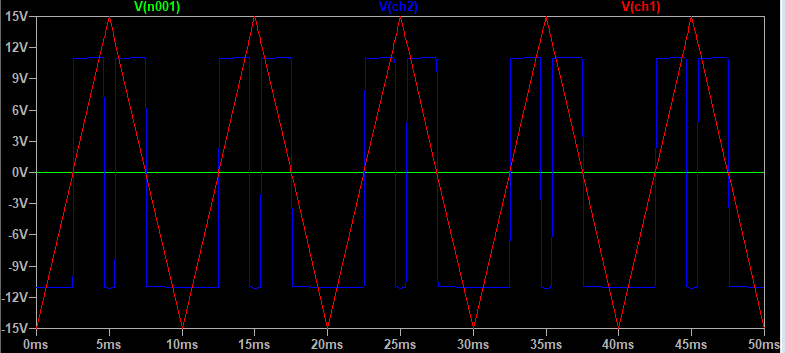
\includegraphics[width=0.9\textwidth]{figures/lab2-1-a.png}
    \caption{Resultado da simulação do item a.}
    \label{fig:figures-lab2-1-a-png}
\end{figure}

\subsubsection*{b)}

O resultado da simulação após a alteração da tensão $V_x$, pode ser vista na figura \ref{fig:figures-lab2-1-b-png}.

\begin{figure}[H]
    \centering
    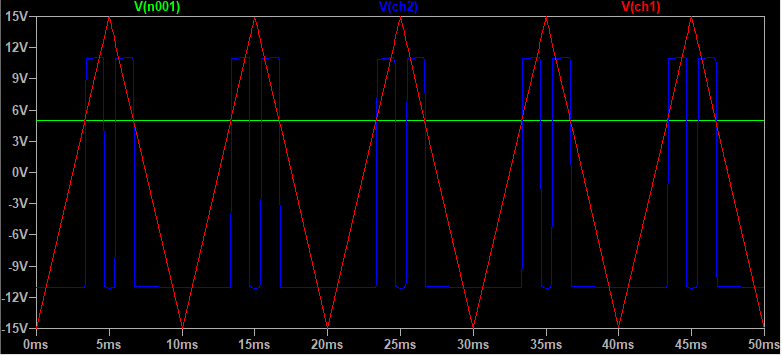
\includegraphics[width=0.9\textwidth]{figures/lab2-1-b.png}
    \caption{Resultado da simulação do item b.}
    \label{fig:figures-lab2-1-b-png}
\end{figure}

\subsubsection*{c)}

O circuito é denominado de comparador porque a saída ($CH2$) apresenta apenas dois valores possíveis: $+V_{cc}$ e 0. Nesse sentido, a saída segue as seguintes regras:
\begin{itemize}
    \item $CH2=0$, caso a tensão de entrada ($CH1$) seja menor que o valor de referência ($V_x$);
    \item $CH2=+V_{cc}$, caso a tensão de entrada ($CH1$) seja maior que o valor de referência ($V_x$);
    \item $CH2=0$, caso a tensão de entrada ($CH1$) seja maior que a tensão de alimentação ($+V_{cc}$).
\end{itemize}
\subsection*{Circuito 2}

Conforme instruído, o circuito foi montado como na figura \ref{fig:figures-lab2-2-circuito-png}.

\begin{figure}[H]
    \centering
    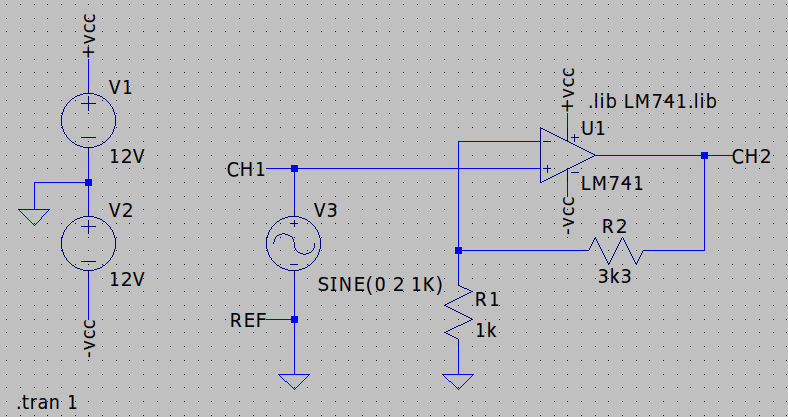
\includegraphics[width=0.8\textwidth]{figures/lab2-2-circuito.png}
    \caption{Segundo circuito do roteiro.}
    \label{fig:figures-lab2-2-circuito-png}
\end{figure}

\subsubsection*{a)}

O resultado da simulação pode ser verificado na figura \ref{fig:figures-lab2-2-a-png}. Conforme visível através do cursor, a tensão de saída respeita, aproximadamente, a relação teórica \[
V_{out}= \left( 1+\frac{3k3}{1k} \right)V_{in} = 8,6 V_p
\] 

\begin{figure}[H]
    \centering
    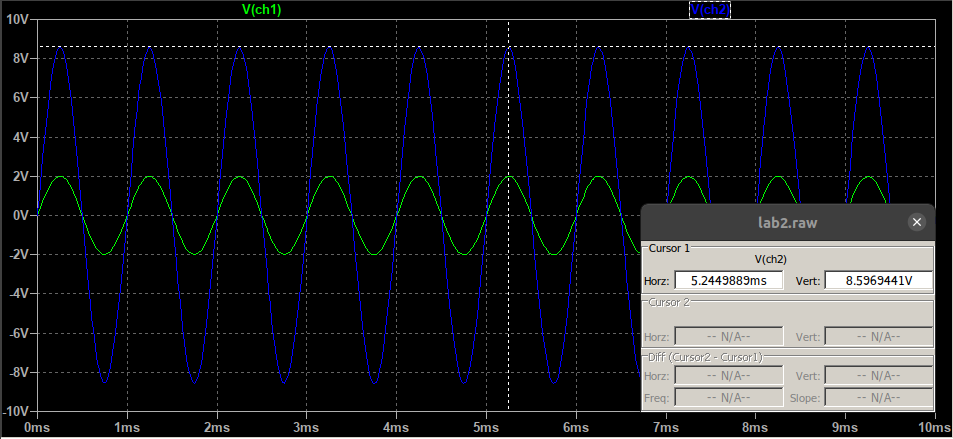
\includegraphics[width=0.8\textwidth]{figures/lab2-2-a.png}
    \caption{Formas de onda da tensão de entrada \emph{V(ch1)} e tensão de saída \emph{V(ch2)}.}
    \label{fig:figures-lab2-2-a-png}
\end{figure}

\subsubsection*{b)}

Para o valor de ganho desejado, precisamos que \[
\frac{R_2}{R_1} = 2 \implies R_2 = 2k\Omega
.\] Podemos ver no resultado, através da figura \ref{fig:figures-lab2-2-b-png}, que a relação teórica é uma boa aproximação.

\begin{figure}[H]
    \centering
    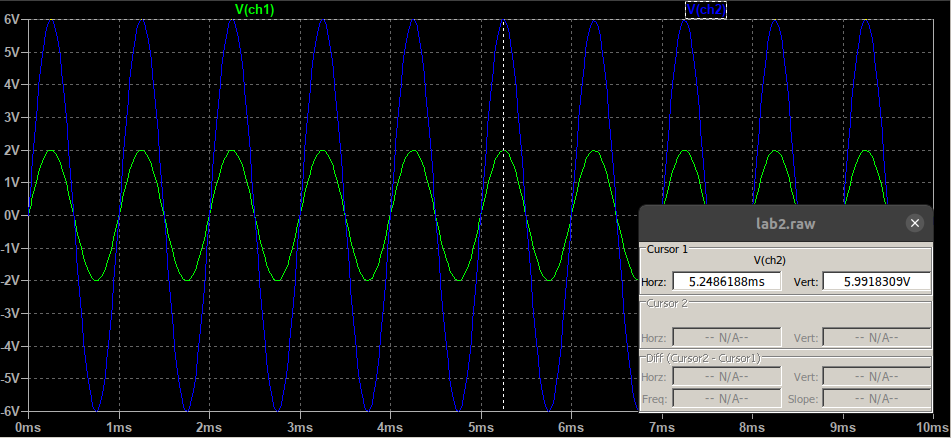
\includegraphics[width=0.8\textwidth]{figures/lab2-2-b.png}
    \caption{Formas de onda do segundo circuito após ajuste de $R_2$.}
    \label{fig:figures-lab2-2-b-png}
\end{figure}

\subsubsection*{c)}

Para determinar o valor real de saturação da saída, o resistor $R_2$ foi incrementado para que se tornasse visível uma saturação na forma de onda monitorada, conforme visível na figura \ref{fig:figures-lab2-2-c-png}. Pelo valor encontrado, podemos calcular o valor da resistência pela relação dos valores de pico \[
    V_{out} = 10,90 = \left( 1 +\frac{R_2}{1k}\right) 2 \implies R_2 = 4k45 \Omega
.\] 

\begin{figure}[H]
    \centering
    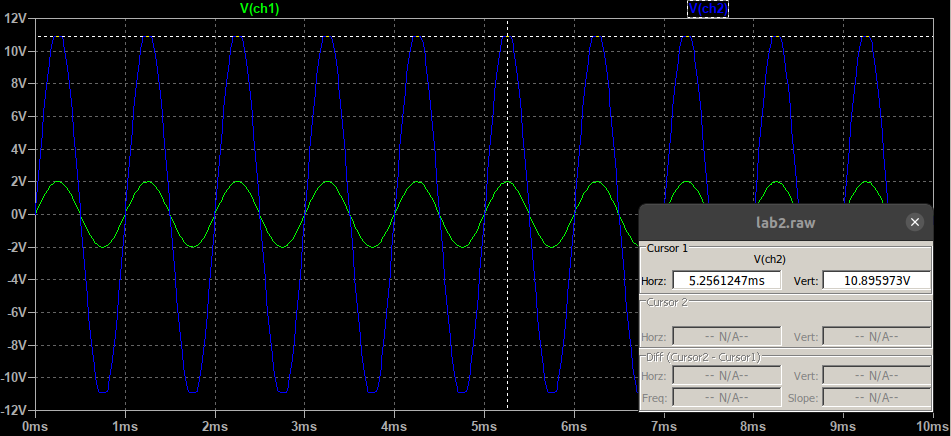
\includegraphics[width=0.8\textwidth]{figures/lab2-2-c.png}
    \caption{Saturação da saída do circuito.}
    \label{fig:figures-lab2-2-c-png}
\end{figure}

\subsubsection*{d)}

Com um sinal de entrada de $2 V_{pp}$ dificilmente o amplificador entraria em uma zona de não linearidade do ganho, então manteria a relação teórica entrada-saída verificada na parte a). Com isso, os resultados de b) se mantém, uma vez que o ganho deriva dessa relação. Finalmente, a resposta de c) provavelmente mudaria uma vez que a tensão de saída, para um mesmo ganho, seria muito menor, ou seja, temos uma margem maior de ganho sem que haja distorção do sinal de saída.

\section*{Conclusão}

Os resultados do circuito comparador apresentou as características desse arranjo, principalmente a alternação entre os dois níveis possíveis de saída a partir dos valores de referência, entrada e alimentação.

A simulação do arranjo como amplificador de sinal mostrou uma proximidade do componente simulado com o componente teórico quanto à relação entrada-saída, ainda que a faixa de saturação do sinal de saída seja muito menor do que no componente teórico.

\end{document}
